
\documentclass[10pt,letterpaper]{article}

\usepackage[letterpaper,margin=0.70in,headheight=22pt,headsep=16pt,footskip=24pt]{geometry}
\usepackage[T1]{fontenc}
\usepackage[utf8]{inputenc}
\usepackage{lmodern}
\usepackage{microtype}
\usepackage{xcolor}
\usepackage{graphicx}
\usepackage{booktabs}
\usepackage{array}
\usepackage{tabularx}
\usepackage{longtable}
\usepackage{amsmath,amssymb}
\usepackage{tikz}
\usetikzlibrary{arrows.meta,positioning,calc,shapes.geometric,decorations.pathreplacing,fit}
\usepackage{enumitem}
\usepackage{fancyhdr}
\usepackage{titlesec}
\usepackage{caption}
\usepackage{listings}
\usepackage{xurl}
\usepackage[hidelinks]{hyperref}
\usepackage{lastpage}
\usepackage{float}
\usepackage{placeins}

\definecolor{FStatRed}{HTML}{A00000}
\definecolor{FStatGray}{HTML}{555555}
\definecolor{FStatBlue}{HTML}{144E8C}
\definecolor{LightGray}{HTML}{F3F3F3}
\definecolor{MidGray}{HTML}{D9D9D9}
\definecolor{DarkText}{HTML}{1A1A1A}
\definecolor{GoodGreen}{HTML}{2B7A2B}
\definecolor{WarnOrange}{HTML}{A65E00}

\renewcommand{\familydefault}{\sfdefault}
\setlength{\parindent}{0pt}
\setlength{\parskip}{5pt}
\renewcommand{\arraystretch}{1.15}
\sloppy
\setlist[itemize]{leftmargin=1.2em,itemsep=2pt,topsep=2pt}
\setlist[enumerate]{leftmargin=1.4em,itemsep=2pt,topsep=2pt}

\titleformat{\section}{\Large\bfseries\color{DarkText}}{}{0pt}{}[\vspace{-3pt}\color{FStatRed}\titlerule]
\titleformat{\subsection}{\large\bfseries\color{DarkText}}{}{0pt}{}
\titleformat{\subsubsection}{\normalsize\bfseries\color{DarkText}}{}{0pt}{}

\newcommand{\code}[1]{\texttt{\detokenize{#1}}}
\newcommand{\apicode}[1]{\texttt{\detokenize{#1}}}
\newcommand{\yes}{\textcolor{GoodGreen}{Yes}}
\newcommand{\no}{\textcolor{FStatGray}{No}}
\newcolumntype{Y}{>{\raggedright\arraybackslash}X}
\newcolumntype{L}[1]{>{\raggedright\arraybackslash}p{#1}}
\newcolumntype{C}[1]{>{\centering\arraybackslash}p{#1}}
\captionsetup{font=small,labelfont=bf}

\lstdefinestyle{shell}{
  basicstyle=\ttfamily\footnotesize,
  breaklines=true,
  columns=fullflexible,
  frame=single,
  rulecolor=\color{MidGray},
  backgroundcolor=\color{LightGray},
  keepspaces=true,
  showstringspaces=false
}
\lstdefinestyle{cstyle}{
  basicstyle=\ttfamily\footnotesize,
  breaklines=true,
  columns=fullflexible,
  frame=single,
  rulecolor=\color{MidGray},
  backgroundcolor=\color{LightGray},
  keepspaces=true,
  showstringspaces=false
}
\lstset{style=shell}

\newcommand{\notebox}[1]{%
  \vspace{4pt}\noindent\fcolorbox{FStatBlue}{LightGray}{%
  \begin{minipage}{0.965\linewidth}%
  \textbf{Note:} #1%
  \end{minipage}}\vspace{4pt}}

\newcommand{\importantbox}[1]{%
  \vspace{4pt}\noindent\fcolorbox{FStatRed}{LightGray}{%
  \begin{minipage}{0.965\linewidth}%
  \textbf{Important:} #1%
  \end{minipage}}\vspace{4pt}}

\newcommand{\field}[1]{\texttt{\detokenize{#1}}}
\newcommand{\dB}{\,\mathrm{dB}}


\pagestyle{fancy}
\fancyhf{}
\fancyhead[L]{\small PilotProxy-UG001}
\fancyhead[C]{\small CUDA F-Statistic DTV Pilot Detector v0.2.0.dev0}
\fancyhead[R]{\small User Guide}
\fancyfoot[L]{\small PilotProxy-UG001 v1.6}
\fancyfoot[C]{\small Pilot-informed DTV detector}
\fancyfoot[R]{\small Page \thepage\ of \pageref{LastPage}}
\renewcommand{\headrulewidth}{0.8pt}
\renewcommand{\headrule}{\hbox to\headwidth{\color{FStatRed}\leaders\hrule height \headrulewidth\hfill}}
\renewcommand{\footrulewidth}{0.8pt}
\renewcommand{\footrule}{\hbox to\headwidth{\color{FStatRed}\leaders\hrule height \footrulewidth\hfill}}

\title{PilotProxy CUDA F-Statistic DTV Pilot Detector v0.2.0.dev0\\User Guide}
\author{West Virginia University}
\date{PilotProxy-UG001 v1.6 \\ July 19, 2026}

\begin{document}
\thispagestyle{empty}
\begin{tikzpicture}[remember picture,overlay]
  \draw[FStatRed,line width=2pt] ($(current page.north west)+(0.72in,-0.35in)$) -- ($(current page.north east)+(-0.72in,-0.35in)$);
  \draw[FStatRed,line width=1pt] ($(current page.south west)+(0.72in,0.45in)$) -- ($(current page.south east)+(-0.72in,0.45in)$);
\end{tikzpicture}
\vspace*{0.25in}
{\fontsize{30}{32}\selectfont\bfseries\color{FStatRed}PilotProxy}\par
\vspace{0.12in}
{\fontsize{23}{26}\selectfont\bfseries CUDA F-Statistic DTV Pilot Detector v0.2.0.dev0}\par
\vspace{0.08in}
{\Large User Guide}\par
\vspace{0.35in}
{\large PilotProxy-UG001 v1.6}\par
{\large July 19, 2026}\par
\vfill
\begin{tabularx}{\linewidth}{|>{\bfseries}L{0.25\linewidth}|Y|}
\hline
Document scope & Package installation, source-tree CUDA build, ATSC waveform generation, detector tests, receiver integration, and interpretation of fixed-point outputs.\\ \hline
Package version & \code{pilot-proxy} v0.2.0.dev0 (unreleased).\\ \hline
Primary runtime controls & A physical channel or pilot frequency selects weights. Frame size and, for synthetic threshold tests, DTV data-shelf SNR control the detector run.\\ \hline
CHIME/CANFAR mode & The CHIME path masks at $F>\mu_0$, where $\mu_0$ is fixed by the quantized weight norms. It does not use a mean estimated from CANFAR data.\\ \hline
Project affiliation & West Virginia University.\\ \hline
\end{tabularx}
\newpage

\section*{Revision History}
\begin{tabularx}{\linewidth}{|L{0.18\linewidth}|L{0.14\linewidth}|Y|}
\hline
\textbf{Date} & \textbf{Version} & \textbf{Revision}\\ \hline
July 19, 2026 & 1.6 & Corrected package state, detection output fields, receiver-metadata consumers, frame-size handling, installation prerequisites, backend labeling, and result-schema coverage. Distinguished the raw $F>1$ convention from the current norm-corrected $F>\mu_0$ CHIME rule.\\ \hline
July 3, 2026 & 1.5 & Updated for the \code{pilot-proxy} 0.2.0 development series. Added installed-package command forms and \code{evaluate-snr --detector-backend cpu-reference}; documented packaged resources and the source-tree CUDA build.\\ \hline
July 2, 2026 & 1.4 & Norm-corrected positive-excess mask ($F>\mu_0$, exact integer form); LaTeX-styled figures with vector-PDF export; publication-analysis commands (\code{inject-pilot-tone}, \code{analyze-injection-recovery}, \code{analyze-cleaning-tradeoff}).\\ \hline
May 29, 2026 & 1.3 & Added receiver-profile integration workflow, full stream-map example, and profile-driven weight generation.\\ \hline
May 29, 2026 & 1.2 & Regenerated for standalone \code{pilot-proxy} v0.1.0.  Added release-candidate CLI names, physical-channel support, strict JSON reporting, calibration field names, and channel-21 edge-wrap handling.\\ \hline
May 29, 2026 & 1.1 & Standalone DTV user guide.  Instrument-specific content removed.\\ \hline
May 29, 2026 & 1.0 & Initial CUDA F-statistic kernel user guide.\\ \hline
\end{tabularx}
\newpage

\setcounter{tocdepth}{1}
\tableofcontents
\clearpage

\section{Introduction}

PilotProxy measures ATSC 1.0 pilot tones with a fixed-point CUDA F-statistic detector. We use the narrow pilot as a proxy for a DTV data shelf that may lie below the broadband noise floor. The standalone testbench generates its own waveform and receiver geometry. The CHIME workflow instead receives instrument metadata and packed baseband data through a separate adapter.

This separation is intentional. The kernel measures target and reference powers without knowing about physical channels, decibels, or telescope layout. Host software supplies those meanings and records them with the output.

\subsection{Detector Objective}

\begin{quote}
Given a local ATSC pilot excess, estimate the equivalent ATSC 1.0 data-shelf SNR relative to the stated non-DTV reference floor.
\end{quote}

We first build and test the detector. We then generate an ATSC waveform, audit the waveform, add noise at a requested shelf SNR, quantize the samples, and run the detector. The final sections describe receiver integration, output fields, limitations, and common failures.

\subsection{Package Contents}

\begin{longtable}{|L{0.30\linewidth}|L{0.62\linewidth}|}
\hline
\textbf{Path} & \textbf{Contents}\\ \hline
\code{cuda/} & CUDA kernel, public C header, CPU reference model, and C/CUDA tests.\\ \hline
\code{src/pilot_proxy/} & Python package for kernel loading, detector geometry, reference channelization, DTV unit conversion, channel helpers, and detection.\\ \hline
\code{src/pilot_proxy/testbench/} & GNU Radio ATSC generation, waveform audit, AWGN injection, quantization, and SNR evaluation.\\ \hline
\code{weights/} & Prebuilt ATSC reference detector weights for channels 14-36.\\ \hline
\code{docs/} & Markdown definitions, data sheet, and user guide source.\\ \hline
\code{examples/quickstart.sh} & End-to-end release sanity-check workflow.\\ \hline
\end{longtable}

\section{Definitions}

The detector compares one target power with two local reference powers. For one result, we compute
\begin{equation}
  F=\frac{2P_t}{P_{r1}+P_{r2}},\qquad \rho=F-1.
\end{equation}
The quantity \(10\log_{10}F\) is the F-statistic level. It is not a physical pilot-to-noise ratio because the basic uncorrected no-excess point is \(F=1\); in that raw convention, positive excess begins at \(F>1\). The current CHIME mask uses the norm-corrected point \(F>\mu_0\) instead, as described in Section~\ref{sec:thresholds}.

The one-bin pilot-excess PNR is:
\begin{equation}
  \mathrm{PNR}_{\mathrm{bin},dB}=10\log_{10}(F-1).
\end{equation}
We convert the one-bin excess to an equivalent DTV data-shelf SNR with
\begin{equation}
  \mathrm{SNR}_{\mathrm{shelf},dB} = \mathrm{PNR}_{\mathrm{bin},dB}
  -10\log_{10}(B_{\mathrm{DTV}}/B_{\mathrm{bin}})
  +\mathrm{pilot\_below\_data\_db}
  -10\log_{10}(\eta_p).
\end{equation}
For the checked-in reference geometry,
\begin{equation}
  B_{\mathrm{bin}}=\frac{400\,\mathrm{MHz}}{1024\times128}=3051.7578125\,\mathrm{Hz},
\end{equation}
which gives the bandwidth spreading term
\begin{equation}
  10\log_{10}(6\,\mathrm{MHz}/B_{\mathrm{bin}})=32.936\dB.
\end{equation}

\notebox{We independently recomputed this conversion from the checked-in formulas. A 1 dB F-statistic level gives \(F=1.2589\), \(\rho=0.2589\), \(\mathrm{PNR}_{\mathrm{bin}}=-5.868\dB\), and \(\mathrm{SNR}_{\mathrm{shelf}}\approx -27.50\dB\) for the 3.052 kHz reference bin.}


\begin{figure}[H]
\centering
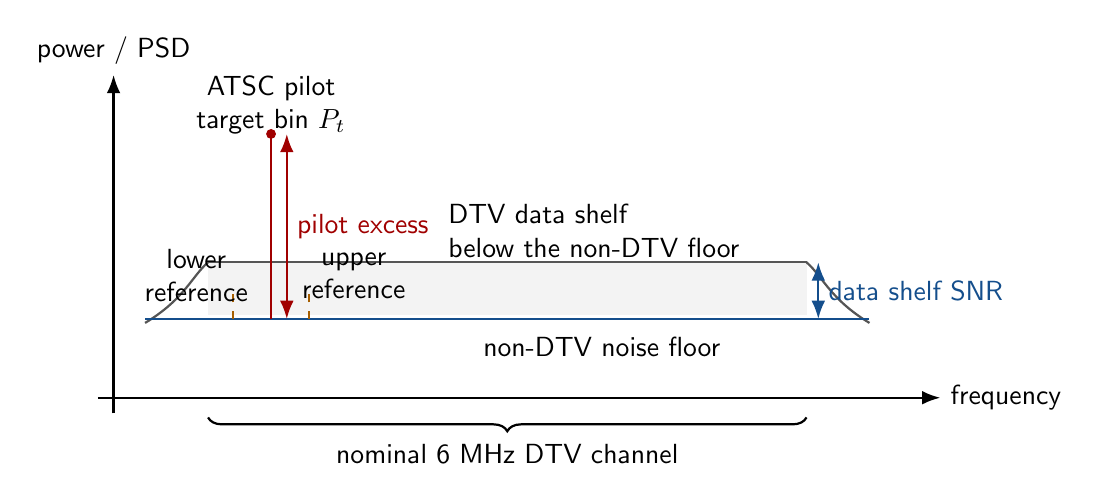
\begin{tikzpicture}[x=1.0cm,y=1.0cm,>=Latex]
  \draw[->,thick] (-0.2,0) -- (10.5,0) node[right]{frequency};
  \draw[->,thick] (0,-0.2) -- (0,4.1) node[above]{power / PSD};
  \draw[fill=LightGray,draw=none] (1.2,1.05) rectangle (8.8,1.72);
  \draw[thick,FStatGray] (1.2,1.72) -- (8.8,1.72);
  \draw[thick,FStatGray] (0.4,0.95) .. controls (0.9,1.25) and (1.0,1.55) .. (1.2,1.72);
  \draw[thick,FStatGray] (8.8,1.72) .. controls (9.0,1.55) and (9.1,1.25) .. (9.6,0.95);
  \draw[thick,FStatBlue] (0.4,1.0) -- (9.6,1.0);
  \draw[thick,FStatRed] (2.0,1.0) -- (2.0,3.35);
  \draw[fill=FStatRed,draw=FStatRed] (2.0,3.35) circle (0.055);
  \draw[dashed,thick,WarnOrange] (1.52,1.0) -- (1.52,1.35);
  \draw[dashed,thick,WarnOrange] (2.48,1.0) -- (2.48,1.35);
  \draw[<->,thick,FStatRed] (2.20,1.0) -- (2.20,3.35) node[midway,right]{pilot excess};
  \draw[<->,thick,FStatBlue] (8.95,1.0) -- (8.95,1.72) node[midway,right]{data shelf SNR};
  \draw[decorate,decoration={brace,mirror,amplitude=5pt},thick] (1.2,-0.25) -- (8.8,-0.25)
    node[midway,below=6pt]{nominal 6 MHz DTV channel};
  \node[align=center] at (2.0,3.72) {ATSC pilot\\target bin $P_t$};
  \node[align=center] at (1.05,1.55) {lower\\reference};
  \node[align=center] at (3.05,1.55) {upper\\reference};
  \node[align=left] at (6.1,2.12) {DTV data shelf\\below the non-DTV floor};
  \node[align=left] at (6.2,0.65) {non-DTV noise floor};
\end{tikzpicture}
\caption{Signal definitions used by the detector. The kernel compares a target pilot bin with two local reference bins. Host software converts the resulting one-bin excess to an equivalent 6 MHz data-shelf SNR under the recorded calibration constants.}
\label{fig:spectrum_definitions}
\end{figure}


\section{Installation Model}

Use an editable checkout for the end-to-end workflows in this guide. Install the extras required by the work you intend to run:
\begin{lstlisting}[style=shell]
python -m pip install -e ".[test]"              # CPU-side tests
python -m pip install -e ".[cuda,test,plot]"    # CUDA and plots
pilot-proxy --help
\end{lstlisting}
Built wheels and source distributions include the reference weight bank and the \code{configs/} tree. Default-resource CPU commands such as \code{list-channels} can therefore run outside the repository. The current examples, repository-relative generated paths, helper scripts, and subprocess-backed two-interpreter workflows should be run from a checkout or supplied explicit paths. The CUDA shared library is not included in the Python distribution; build it from a clone before running GPU-backed commands.

\subsection{Python Environments}

When GNU Radio is installed as a system package, two Python interpreters may be necessary:
\begin{itemize}
  \item GNU Radio Python: used for ATSC generation and GNU Radio AWGN, typically \code{/usr/bin/python3}.
  \item CUDA Python: used for CuPy, the CUDA shared library, and detector evaluation --- the repository virtual environment installed with the \code{cuda}, \code{test}, and, when needed, \code{plot} extras.
\end{itemize}

Keep the CUDA environment active for the examples below. The \code{generate-atsc} command and GNU Radio noise source invoke the interpreter supplied through \code{--gnuradio-python}, typically \code{/usr/bin/python3}. PilotProxy must also be importable by that interpreter. The supported guide setup is an editable source checkout, whose wrapper supplies the checkout's \code{src/} path to the child process. If using a wheel instead, install PilotProxy for the GNU Radio interpreter or provide an explicit compatible \code{PYTHONPATH}; installing it only in the CUDA environment is not sufficient. On WSL, the CUDA driver path is commonly \code{/usr/lib/wsl/lib}; verify it on the target host.

On WSL, adding the Python environment's \code{lib/} directory to
\code{LD_LIBRARY_PATH} can make \code{/usr/bin/bash} load that environment's
\code{libtinfo.so.6} and print a \code{no version information available}
warning. The examples require only the CUDA driver path. Pass
\code{--no-python-user-site} to \code{generate-atsc} when user-site packages shadow the NumPy build used by GNU Radio; the evaluator's GNU Radio noise subprocess already disables the user site.

\section{Build and Test}

\subsection{Build the CUDA Kernel}

Build for the target GPU architecture:
\begin{lstlisting}[style=shell]
make build-kernel   # SM auto-detected; pass SM=<arch> to override
\end{lstlisting}
This builds \code{cuda/libfstatistic.so} and stages a copy to:
\begin{lstlisting}[style=shell]
~/.cache/pilot_proxy/libfstatistic.so
\end{lstlisting}
On WSL, the cached copy avoids loading the shared library directly from \code{/mnt/c}.  If you rebuild only under \code{cuda/}, remove the staged copy with:
\begin{lstlisting}[style=shell]
make clean-cache
\end{lstlisting}

\subsection{Run Tests}

Run Python tests:
\begin{lstlisting}[style=shell]
python -m pytest tests -q
\end{lstlisting}
Run CUDA/kernel tests on a CUDA-capable host:
\begin{lstlisting}[style=shell]
make -C cuda test DP4A=1   # SM auto-detected
\end{lstlisting}
The repository separates Python, CPU, CUDA, and GNU Radio checks. Record the commit, host, and commands for each release test. A Python-only result does not establish CUDA or GNU Radio behavior, so run those checks on a suitable target before tagging a release.

\section{Quickstart}

The provided script exercises the main standalone path:
\begin{lstlisting}[style=shell]
bash examples/quickstart.sh   # GPU architecture auto-detected
\end{lstlisting}
The output includes a waveform audit, detector-input generation, an SNR evaluation, and detection JSON. The current summary headings are shown below. Numeric rows are intentionally omitted here; rerun the script on the target commit and treat that recorded output as the result.
\begin{lstlisting}[style=shell]
frequency_offset_hz, requested_snr_shelf_db,
measured_truth_snr_shelf_db, cpu_float_snr_shelf_db,
gpu_snr_shelf_db, gpu_snr_error_db
...
blocks, positive_excess_set, fstat_raw_mean,
estimated_snr_shelf_db_mean
...
\end{lstlisting}

\section{Generate and Audit an ATSC Waveform}

\subsection{Generate a Reference ATSC Signal}

Generate the reference ATSC waveform. GNU Radio runs under the interpreter given by \code{--gnuradio-python}:
\begin{lstlisting}[style=shell]
pilot-proxy generate-atsc \
  --gnuradio-python /usr/bin/python3 \
  --output-iq generated/atsc/atsc_8vsb_complex64.cfile \
  --num-iq-samples 600000
\end{lstlisting}

\subsection{Audit the Reference Waveform}

Audit the generated waveform before detector evaluation:
\begin{lstlisting}[style=shell]
pilot-proxy audit-atsc \
  --input-iq generated/atsc/atsc_8vsb_complex64.cfile
\end{lstlisting}
The audit records the pilot frequency, pilot-to-data power, occupied bandwidth, shelf flatness, and edge rolloff. The field \field{measured_pilot_to_data_power_db} is the signed quantity \(10\log_{10}(P_{\mathrm{pilot}}/P_{\mathrm{data}})\). The field \field{measured_pilot_below_data_db} records its positive magnitude when the pilot is below the data shelf.

\notebox{The audit reports pilot frequency in the generated complex-baseband coordinate.  For physical channel 14, the baseband pilot corresponds to an RF pilot at 470.309441 MHz after reference-band placement.}

\section{Reference Channelizer and Detector Resolution}

The standalone testbench uses the following polyphase filter-bank (PFB) reference front end:
\begin{longtable}{|L{0.36\linewidth}|L{0.56\linewidth}|}
\hline
\textbf{Quantity} & \textbf{Value}\\ \hline
Real ADC sample rate & 800 MS/s \\ \hline
Reference lower band edge & 400 MHz \\ \hline
Reference bandwidth & 400 MHz \\ \hline
PFB taps & 4 \\ \hline
PFB FFT size & 2048 real-input samples \\ \hline
Usable positive-frequency channels & 1024 \\ \hline
Coarse-channel spacing & 390.625 kHz \\ \hline
Detector window & 128 samples \\ \hline
Fine detector-bin width & 3051.7578125 Hz \\ \hline
\end{longtable}
This geometry gives a 3051.7578125 Hz fine-bin width. The default pilot-to-shelf conversion is valid for this stated geometry; another receiver must supply its measured or modeled effective noise bandwidth.

\section{Channel Selection}

List physical channels supported by the shipped weight bank:
\begin{lstlisting}[style=shell]
pilot-proxy list-channels
\end{lstlisting}
The included weights cover physical channels 14 through 36. The frequency helpers accept other UHF channels, but the detector still requires a matching row in the weight manifest. The standalone ascending-frequency reference coordinate places channels 14, 21, and 36 at coarse indices 179, 287, and 517. The shipped post-spectral-sense-normalization CHIME manifest, which \code{list-channels} reports, stores the same targets at 843, 735, and 505. Do not compare an index without naming its coordinate system.

The default channel is physical channel 14:
\begin{equation}
  f_{\mathrm{lower}}=470\,\mathrm{MHz},\quad f_{\mathrm{pilot}}=470.309441\,\mathrm{MHz},\quad f_{\mathrm{center}}=473\,\mathrm{MHz}.
\end{equation}
Physical channel 21 tests a coarse-channel boundary. Its weight row wraps the lower reference across the circular coarse-channel spectrum while preserving the requested \(-2,+2\) fine-bin offsets. The manifest records this choice with \field{adaptive_reference_placement=true}.

\section{Quantize and Create Detector Input}

Create a packed detector matrix:
\begin{lstlisting}[style=shell]
pilot-proxy quantize \
  --input-iq generated/atsc/atsc_8vsb_complex64.cfile \
  --physical-channel 14 \
  --frame-size-samples 16384
\end{lstlisting}
This example uses a 16,384-sample frame because that is the checked-in reference test profile. The same value also represents the planned CHIME Engine upgrade interface used by this repository. It is not a statement about the currently deployed CHIME correlator. The software does not infer one universal frame size from HDF5 metadata: set \code{chime-run --frame-size-samples} from verified product information, and set the DataTrawl instrument \code{nfft} used by \code{chime-scan}. Record the resolved value with each real-data product.

The output matrix is row-major and has shape \code{(rows, 128)} or \code{(batch, rows, 128)} with dtype \code{int8}. The CUDA wrapper checks both properties before passing pointers to the kernel.

\section{Evaluate Shelf-SNR Response}

Run the synthetic evaluator with the CUDA backend. This example shows the WSL driver path:
\begin{lstlisting}[style=shell]
LD_LIBRARY_PATH=/usr/lib/wsl/lib \
pilot-proxy evaluate-snr \
  --input-iq generated/atsc/atsc_8vsb_complex64.cfile \
  --physical-channel 14 \
  --frame-size-samples 16384 \
  --requested-snr-shelf-db -26 \
  --threshold-snr-shelf-db -26 \
  --noise-trials 10 \
  --noise-source gnuradio \
  --gnuradio-python /usr/bin/python3
\end{lstlisting}
Outputs are written under \code{generated/dtv_snr_eval/}:
\begin{itemize}
  \item \code{dtv_snr_eval.csv}: per-trial validation rows;
  \item \code{dtv_snr_summary.csv}: grouped summary;
  \item \code{dtv_snr_eval.json}: full strict-JSON validation report.
\end{itemize}

If neither explicit \code{--requested-snr-shelf-db} values nor an
\code{--snr-start-db}/\code{--snr-stop-db}/\code{--snr-step-db} range is
provided, the evaluator sweeps from \(-60\dB\) to \(0\dB\) in 3 dB steps.
Each \code{--noise-trials} entry adds one independently generated noise frame
at every requested SNR and frequency offset. Use several trials per point when
the objective is a response curve. The GNU Radio noise path exercises more of
the reference signal chain, while the Python noise path reduces runtime for a
large sweep:
\begin{lstlisting}[style=shell]
LD_LIBRARY_PATH=/usr/lib/wsl/lib \
pilot-proxy evaluate-snr \
  --input-iq generated/atsc/atsc_8vsb_complex64.cfile \
  --physical-channel 14 \
  --frame-size-samples 16384 \
  --num-input-streams 1 \
  --threshold-snr-shelf-db -26 \
  --noise-trials 10 \
  --noise-source python
\end{lstlisting}
This configuration produces 210 detector frames: 10 frames at each of 21 SNR
values. Ten trials are useful for checking the workflow but do not by themselves
support a publication uncertainty claim. Choose the final trial count from the
precision required for the plotted interval and record that choice. Add
\code{--standard-frequency-offset-sweep} when the \(-1\mathrm{kHz}\),
\(0\mathrm{Hz}\), and \(+1\mathrm{kHz}\) curves are needed; this triples the
number of evaluated offset conditions.

Large sweeps do not require a GPU. With \code{--detector-backend cpu-reference}, the primary fields come from the integer CPU reference and each row records the backend. Before interpreting a CPU-only sweep as representative of the CUDA implementation, compare a small same-seed sample across both backends as described in \code{docs/PUBLICATION_VALIDATION.md}:
\begin{lstlisting}[style=shell]
pilot-proxy evaluate-snr \
  --input-iq generated/atsc/atsc_8vsb_complex64.cfile \
  --physical-channel 14 \
  --frame-size-samples 16384 \
  --num-input-streams 1 \
  --threshold-snr-shelf-db -26 \
  --noise-trials 300 \
  --noise-source python \
  --detector-backend cpu-reference
\end{lstlisting}

For a CUDA-backed sweep, render the grouped result without plot smoothing:
\begin{lstlisting}[style=shell]
pilot-proxy plot-results
\end{lstlisting}
The CSV, JSON, and PNG use the same grouped summary values. The current plot helper hard-labels its selected fixed-point series ``GPU fixed-point.'' Do not use that label for a \code{cpu-reference} result: plot the CSV directly or relabel the series ``CPU fixed-point,'' and retain the recorded \field{detector_backend} with the figure.

\begin{figure}[H]
\centering
\IfFileExists{../generated/dtv_snr_eval/dtv_snr_sweep.png}{%
\includegraphics[width=0.92\linewidth]{../generated/dtv_snr_eval/dtv_snr_sweep.png}
\caption{Example shelf-SNR response for the stated synthetic configuration: \(-60\dB\) to \(0\dB\) in 3 dB steps, 10 Python-noise trials per point, one input stream, and no smoothing. The diagonal is an input-equals-output reference. The curves compare the unquantized floating-point model with the selected packed-int4 fixed-point backend. Ten trials per point demonstrate the workflow but do not define the uncertainty of a publication result.}
}{%
\fbox{\parbox{0.86\linewidth}{\centering The optional generated SNR sweep figure was not found. Run the validation sweep and plot workflow to create \code{generated/dtv_snr_eval/dtv_snr_sweep.png}.}}
\caption{Example shelf-SNR response for the stated synthetic configuration: \(-60\dB\) to \(0\dB\) in 3 dB steps, 10 Python-noise trials per point, one input stream, and no smoothing. The diagonal is an input-equals-output reference. The curves compare the unquantized floating-point model with the selected packed-int4 fixed-point backend. Ten trials per point demonstrate the workflow but do not define the uncertainty of a publication result.}
}
\label{fig:snr_sweep_10trial}
\end{figure}

Important report fields include:
\begin{itemize}
  \item \field{requested_snr_shelf_db}
  \item \field{measured_truth_snr_shelf_db}
  \item \field{measured_truth_composite_atsc_snr_db}
  \item \field{p_target_u64}, \field{p_ref_lower_u64}, \field{p_ref_upper_u64}
  \item \field{fstat_raw}, \field{fstat_level_db}, \field{pilot_excess_linear}, \field{pnr_bin_db}
  \item \field{estimated_snr_shelf_db}, \field{snr_error_db}
  \item \field{mask}, when \code{--threshold-snr-shelf-db} is supplied.
\end{itemize}


\begin{figure}[H]
\centering
% Shared architecture diagram: the standalone validation flow.
% Single source of truth -- \input by PilotProxy_DS001 (Data Sheet) and
% PilotProxy_UG001 (User Guide), and rendered to validation_flow.svg for
% README.md. Requires: tikz libraries arrows.meta + positioning, and the
% colors FStatBlue (#144E8C) and LightGray (#F3F3F3) defined by the host
% document (or by validation_flow_standalone.tex when rendering the svg).
% Re-render the svg after editing:
%   cd docs/figures && pdflatex validation_flow_standalone.tex \
%     && pdftocairo -svg validation_flow_standalone.pdf validation_flow.svg
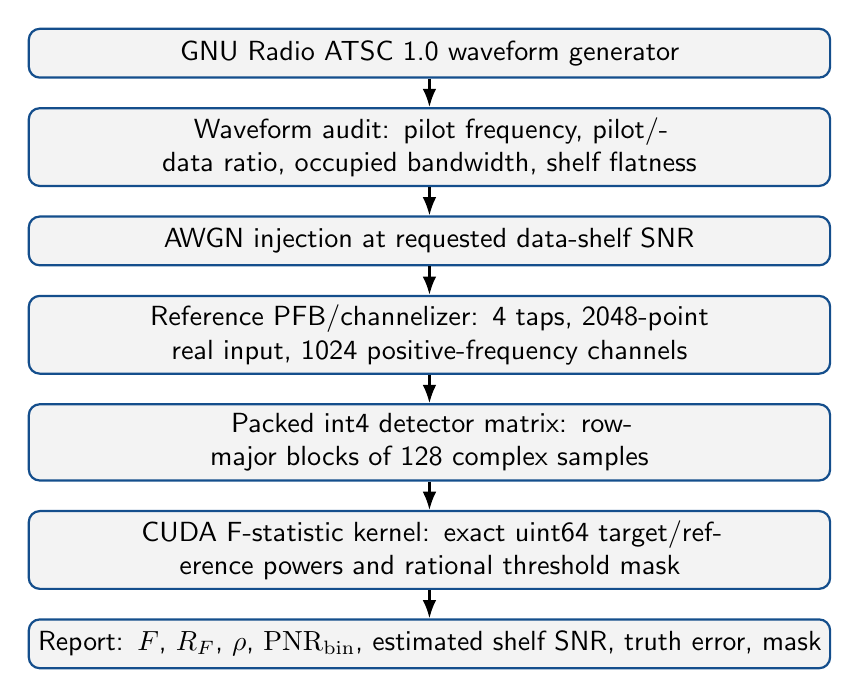
\begin{tikzpicture}[node distance=0.36cm,>=Latex]
\tikzstyle{block}=[rectangle,rounded corners,draw=FStatBlue,thick,fill=LightGray,minimum height=0.62cm,text width=0.82\linewidth,align=center]
\node[block] (a) {GNU Radio ATSC 1.0 waveform generator};
\node[block,below=of a] (b) {Waveform audit: pilot frequency, pilot/data ratio, occupied bandwidth, shelf flatness};
\node[block,below=of b] (c) {AWGN injection at requested data-shelf SNR};
\node[block,below=of c] (d) {Reference PFB/channelizer: 4 taps, 2048-point real input, 1024 positive-frequency channels};
\node[block,below=of d] (e) {Packed int4 detector matrix: row-major blocks of 128 complex samples};
\node[block,below=of e] (f) {CUDA F-statistic kernel: exact uint64 target/reference powers and rational threshold mask};
\node[block,below=of f] (g) {Report: $F$, $R_F$, $\rho$, $\mathrm{PNR}_{\mathrm{bin}}$, estimated shelf SNR, truth error, mask};
\draw[->,thick] (a) -- (b);
\draw[->,thick] (b) -- (c);
\draw[->,thick] (c) -- (d);
\draw[->,thick] (d) -- (e);
\draw[->,thick] (e) -- (f);
\draw[->,thick] (f) -- (g);
\end{tikzpicture}

\caption{Standalone validation flow. The included reference front end converts a generated ATSC waveform into the packed-input contract used by the detector.}
\label{fig:validation_flow}
\end{figure}


\newpage\section{Detection on a Packed Matrix}

Run detection on a prebuilt packed detector matrix:
\begin{lstlisting}[style=shell]
LD_LIBRARY_PATH=/usr/lib/wsl/lib \
pilot-proxy detect \
  --input-detector-matrix generated/detector_input/detector_matrix_i4.npy
\end{lstlisting}
The command reads the pilot identity from the \code{metadata.json} sidecar that
\code{quantize} writes next to the matrix; an explicit
\code{--physical-channel} or \code{--dtv-pilot-mhz} must agree with it, and
without either a sidecar or a flag, \code{detect} stops because it cannot select a weight row safely.
If \code{detector_matrix_i4.npy} is absent but the batched
\code{detector_blocks_i4.npy} file exists, \code{detect} resolves the default
input to the batched file automatically.  If neither file exists, run
\code{quantize} first.

The detector JSON includes:
\begin{itemize}
  \item \field{selected_weight_layout}
  \item \field{result_schema} with \code{schema_version=pilot_proxy_result_v2}
  \item \field{layout} with \field{frame_size_samples}, \field{num_input_streams}, \field{windows_per_stream}, and \field{detector_rows_per_frame}
  \item \field{mask_rule}, \field{target_norm_sq}, \field{ref_norm_sum_sq}, and \field{mu0}
  \item per-block \field{mask} and \field{positive_excess_mask}, exact powers, \field{fstat_raw}, raw \field{pilot_excess_linear}, norm-corrected \field{pilot_excess_corrected}, and estimated shelf SNR.
\end{itemize}
The current \code{detect} command does not apply a user-supplied shelf-SNR threshold. Its threshold fields inside \field{result_schema} are \code{null}, and it masks a valid block at the norm-corrected condition \(F>\mu_0\). The earlier/basic raw convention \(F>1\) remains useful for defining \(\rho=F-1\), but it is not the current CHIME mask rule.

\section{Receiver Integration Contract}

The kernel does not encode telescope metadata. Receiver integrations provide the following JSON records and arrays:
\begin{itemize}
  \item \code{configs/detector_core/pilotproxy_cuda_fstat_v1.json} describes the locked CUDA kernel contract.
  \item \code{receiver_profile.json} describes RF band, channelizer geometry, spectral sense, frame size, input streams, quantization defaults, bin ENBW, and pilot-capture efficiency.
  \item \code{stream_map.json} maps stream indices to feed, polarization, beam, or other receiver-specific identifiers.
  \item \code{check-profile}, \code{check-layout}, \code{make-weights}, and \code{chime-run} consume the applicable profile or stream-map records. The standalone \code{detect} command selects shipped weights from its sidecar or channel flag, while \code{evaluate-snr} uses the fixed testbench geometry.
\end{itemize}

Useful metadata checks:
\begin{lstlisting}[style=shell]
pilot-proxy check-profile \
  --receiver-profile configs/receiver_profiles/reference_800mhz_pfb.json

pilot-proxy check-layout \
  --receiver-profile configs/receiver_profiles/chime_dtv_fengine.json \
  --stream-map configs/stream_maps/chime_feed_pol_example.json
\end{lstlisting}

Generate receiver-profile-backed weights with:
\begin{lstlisting}[style=shell]
pilot-proxy make-weights \
  --receiver-profile configs/receiver_profiles/chime_dtv_fengine.json \
  --detector-core-profile configs/detector_core/pilotproxy_cuda_fstat_v1.json \
  --physical-channel-range 14:36 \
  --weight-coordinate-system post_spectral_sense_normalization \
  --output generated/weights/chime_dtv_weights_k128.bin
\end{lstlisting}

The CHIME profile has status \code{example_requires_data_product_verification}.
Its 16,384-sample frame represents the planned Engine upgrade interface used for
the repository's tests and analysis, not the current deployed correlator. The
example stream map contains 2,048 feed-polarization entries so the layout check
exercises the intended row-count contract. Verify both files against the actual
data product before using them in a telescope run. Neither file is required by
the standalone ATSC testbench.

\section{Thresholds}
\label{sec:thresholds}

For the synthetic threshold path, the user provides \code{threshold_snr_shelf_db}. Host code converts it to a rational half-threshold, after which the kernel compares integer powers and integer threshold terms.


\begin{figure}[H]
\centering
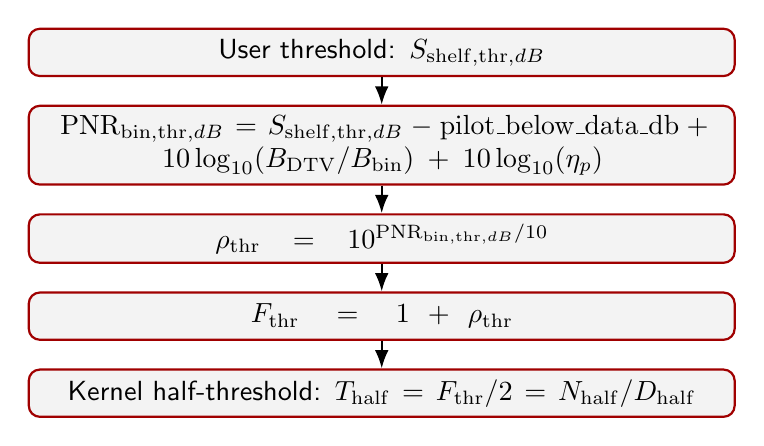
\begin{tikzpicture}[node distance=0.35cm,>=Latex]
\tikzstyle{block}=[rectangle,rounded corners,draw=FStatRed,thick,fill=LightGray,minimum height=0.60cm,text width=0.72\linewidth,align=center]
\node[block] (a) {User threshold: $S_{\mathrm{shelf,thr},dB}$};
\node[block,below=of a] (b) {$\mathrm{PNR}_{\mathrm{bin,thr},dB}=S_{\mathrm{shelf,thr},dB}-\mathrm{pilot\_below\_data\_db}+10\log_{10}(B_{\mathrm{DTV}}/B_{\mathrm{bin}})+10\log_{10}(\eta_p)$};
\node[block,below=of b] (c) {$\rho_{\mathrm{thr}}=10^{\mathrm{PNR}_{\mathrm{bin,thr},dB}/10}$};
\node[block,below=of c] (d) {$F_{\mathrm{thr}}=1+\rho_{\mathrm{thr}}$};
\node[block,below=of d] (e) {Kernel half-threshold: $T_{\mathrm{half}}=F_{\mathrm{thr}}/2=N_{\mathrm{half}}/D_{\mathrm{half}}$};
\draw[->,thick] (a) -- (b);
\draw[->,thick] (b) -- (c);
\draw[->,thick] (c) -- (d);
\draw[->,thick] (d) -- (e);
\end{tikzpicture}
\caption{Synthetic threshold conversion. The user supplies a shelf-SNR threshold, while the kernel receives a fixed-point rational half-threshold.}
\label{fig:threshold_conversion}
\end{figure}


For a \(-26\dB\) shelf-SNR threshold and the included reference geometry, the checked-in conversion code gives
\begin{lstlisting}[style=shell]
threshold_snr_shelf_db       = -26.000
threshold_pnr_bin_db         =  -4.364
threshold_pilot_excess_linear=   0.3661
threshold_fstat_raw          =   1.3661
threshold_half_float         =   0.68305
\end{lstlisting}

The CHIME positive-excess path does not use this user-supplied shelf-SNR
threshold. Int4 quantization makes the target and reference weight norms
slightly unequal, so each weight row has a fixed null point
\begin{equation}
\mu_0=\frac{2\,\lVert w_t\rVert^2}
{\lVert w_{r1}\rVert^2+\lVert w_{r2}\rVert^2}.
\end{equation}
The earlier/basic raw convention calls \(F>1\) positive excess. The current implementation instead masks a valid frame when \(F>\mu_0\), using integer cross
multiplication. We compute \(\mu_0\) from the packed weights; it is not a mean
estimated from CANFAR data. This rule corrects the weight-normalization point,
but it does not supply an empirical false-positive rate or an operational RFI
severity threshold.

\section{Standard and Calibrated Conversion}

The standard synthetic conversion uses
\begin{lstlisting}[style=shell]
--pilot-below-data-db 11.3
--bin-enbw-hz 3051.7578125
--pilot-capture-efficiency 1.0
--dtv-bandwidth-hz 6000000
\end{lstlisting}
The positive field \field{pilot_below_data_db} records how far the pilot power lies below the average data-shelf power. For example, an audit value of \field{measured_pilot_to_data_power_db=-11.9} corresponds to \field{measured_pilot_below_data_db=11.9}.

Use calibrated mode only when a receiver measurement or model supports the overrides:
\begin{lstlisting}[style=shell]
--pilot-below-data-db VALUE
--bin-enbw-hz VALUE
--pilot-capture-efficiency VALUE
\end{lstlisting}
The output report records the values used, so an analysis can reproduce the conversion.

\section{C API Overview}

The public C API is declared in \code{cuda/f_statistic.h}. In this example, \code{d_in}, \code{d_num_out}, \code{d_den_out}, \code{d_mask_out}, and \code{d_overflow_count} are device pointers. The overflow counter must address one device \code{unsigned int}; \code{host_weights} is a host pointer. A typical thresholded call is
\begin{lstlisting}[style=cstyle,language=C]
int K, N, bits, ref_offset;
FStat_GetSpecs(&K, &N, &bits, &ref_offset);

void* h = FStat_Create(d_in, NULL, detector_rows_per_block);
if (h == NULL) {
    /* Read FStat_LastError() and stop. */
    return;
}
FStat_Compute_NumDen_Mask_RationalHalf_WithOverflowCount(
    h,
    host_weights,
    threshold_half_num,
    threshold_half_den,
    d_num_out,
    d_den_out,
    d_mask_out,
    d_overflow_count);
if (FStat_LastError()[0] != 0) {
    /* Handle the recorded CUDA/API error. */
}
FStat_Destroy(h);
\end{lstlisting}
The compute call writes
\begin{equation}
  \mathrm{d\_num\_out}=P_t,\qquad \mathrm{d\_den\_out}=P_{r1}+P_{r2}.
\end{equation}
Host code then computes
\begin{equation}
  F=\frac{2\,\mathrm{num}}{\mathrm{den}}.
\end{equation}
A zero denominator cannot define \(F\). The kernel sets the mask to zero for this case. Unchecked C and Python conversion helpers return zero pilot excess. The checked C helper exposes the invalid denominator; Python callers must inspect \code{den} or \field{p_ref_sum_u64} before interpreting the conversion.

\section{JSON Output Policy}

JSON reports do not emit NaN or infinity; values that are not finite are serialized as \code{null}. CSV files may retain NaN text when analysis software can represent it.

Detector and synthetic SNR-evaluator JSON reports include \field{result_schema} with \code{schema_version=pilot_proxy_result_v2}. This object records the statistic definition, layout, calibration constants, threshold conversion, fixed-point contract, and mask convention needed to interpret those reports. Audit, quantization, summary, injection, and CHIME products use their own documented top-level schemas.

The combined-row statistic is:
\begin{equation}
F = \frac{2\sum_r P_{t,r}}{\sum_r P_{r1,r}+\sum_r P_{r2,r}},
\end{equation}
where \(r\) indexes detector rows. We sum powers first and form one ratio; averaging per-row F-statistics would define a different estimator.

When a product averages masked data, it excludes rejected blocks rather than zero-filling them:
\begin{equation}
\bar{P}_{\mathrm{after}} =
\frac{\sum_b P_b(1-M_b)}{\sum_b (1-M_b)}.
\end{equation}
Here \(M_b=1\) excludes block \(b\).

\section{Result Summaries}

Use the summary helper to reduce a result file to compact CSV and JSON statistics:
\begin{lstlisting}[style=shell]
pilot-proxy summarize-results \
  --input generated/dtv_snr_eval/dtv_snr_eval.json \
  --output-dir generated/summary
\end{lstlisting}
This writes \code{summary.csv} and \code{summary.json}. For an SNR sweep, the
command skips histograms because the input mixes distinct requested-SNR
populations. A histogram is easier to interpret for repeated trials at one
fixed SNR. Use \code{--histograms always} only when that mixed distribution is
intentionally part of the diagnostic.

\section{Known Limitations}

\begin{itemize}
  \item The synthetic testbench models GNU Radio ATSC 1.0 signals. It does not model other broadcast standards or establish telescope performance.
  \item The CHIME real-data workflow (\code{chime-run}, \code{chime-scan}, and the HDF5 reader) is documented in \code{docs/CANFAR_RUNBOOK.md} and \code{docs/PUBLICATION_VALIDATION.md}.
  \item The checked-in CHIME profile and stream map are examples that require data-product verification. The 16,384-sample frame is the planned Engine upgrade profile used by this repository, not a claim about the current deployed frame. \code{chime-run} uses its explicit override, and \code{chime-scan} uses the DataTrawl instrument \code{nfft}; neither path should be described as automatically discovering a universal HDF5 frame size.
  \item Synthetic threshold tests accept a shelf-SNR threshold. The CHIME path instead uses $F>\mu_0$, with \(\mu_0\) fixed by the weight norms. Neither rule is an empirically calibrated telescope false-positive threshold.
  \item Receiver profiles define an adapter contract; they do not establish that a telescope pipeline has been deployed or validated.
  \item Installed packages carry the weight bank and \code{configs/} resources, so default-resource commands can run outside the repository. Repository-relative examples, helper scripts, second-interpreter subprocesses, and the CUDA build require a checkout or explicit paths. The CUDA kernel itself is not packaged and builds from the cloned source tree (\code{make build-kernel}).
\end{itemize}

\section{Troubleshooting}

\subsection{GNU Radio imports fail}
Use the system GNU Radio Python, typically \code{/usr/bin/python3}. Confirm that it can import PilotProxy from the editable checkout or an explicit \code{PYTHONPATH}; a wheel installed only in the CUDA environment is not visible to it. Set \code{PYTHONNOUSERSITE=1} when user-site packages shadow the GNU Radio NumPy build.

\subsection{CUDA shared library not found}
Run \code{make build-kernel SM=<target>} and ensure \code{LD_LIBRARY_PATH} includes the CUDA driver path. On WSL, this is commonly \code{/usr/lib/wsl/lib}; verify the target host and prefer the staged cache copy under \code{~/.cache/pilot_proxy/}.

\subsection{Wrong detector matrix shape}
The packed detector matrix must have dtype \code{int8} and last dimension 128.  Use \code{pilot-proxy quantize} to build the expected format.

\subsection{No weights for channel}
The shipped bank covers physical channels 14-36.  Use \code{pilot-proxy list-channels} to list available targets.

\subsection{PNR is null}
If \(F\leq1\), the raw pilot-excess ratio is non-positive and \(10\log_{10}(F-1)\) is undefined. The JSON value is therefore \code{null}; this can occur for noise-only and weak-signal trials.

\begin{thebibliography}{9}
\bibitem{atsc_a53_part2_2011} Advanced Television Systems Committee, \emph{ATSC Digital Television Standard, Part 2: RF/Transmission System Characteristics}, A/53 Part 2:2011, 15 December 2011. \url{https://www.atsc.org/wp-content/uploads/2021/04/A53-Part-2-2011.pdf}
\bibitem{ecfr_73603} Electronic Code of Federal Regulations, 47 CFR \S 73.603, \emph{Numerical designation of television channels}. \url{https://www.ecfr.gov/current/title-47/chapter-I/subchapter-C/part-73/subpart-E/section-73.603}
\bibitem{gnuradio_dtv} GNU Radio Manual, \emph{DTV/ATSC module documentation}. \url{https://www.gnuradio.org/doc/sphinx-3.7.7.1/atsc/index.html}
\bibitem{gnuradio_noise} GNU Radio Manual, \emph{gr::analog::noise\_source}, complex noise-source amplitude convention. \url{https://www.gnuradio.org/doc/doxygen/classgr_1_1analog_1_1noise__source.html}
\end{thebibliography}

\end{document}
